\documentclass[11pt,twoside,fleqn]{scrreprt}
%\usepackage[utf8x]{inputenc}
%\usepackage[utf8]{inputenc}
\usepackage[T1]{fontenc}
%\usepackage[latin1]{inputenc}
\usepackage{graphicx}
\usepackage[margin=2.0cm,bottom=2.5cm]{geometry}
\usepackage{subfig}
%\usepackage{ulem}
\usepackage{fancyhdr}
\usepackage{hyperref}
\usepackage[usenames,dvipsnames]{color}
%\usepackage{amssymb}
\usepackage{amsmath}
%\usepackage{mathrsfs}
%\usepackage{textgreek}
%\usepackage{curves}
%\usepackage{latexsym} % ein paar Symbole
%\usepackage{textcomp} % ein paar Symbole
%\usepackage{natbib}
\usepackage{ulem}
\usepackage{bm}
%\usepackage{mathtools}
%\usepackage{cancel}
%\usepackage{longtable}
%\usepackage{booktabs}
\usepackage[charter]{mathdesign}
%\usepackage{mathptmx}
\usepackage{url}
\usepackage{multicol}
\usepackage{authblk}
%\usepackage{nomencl}
\usepackage{makeidx}
\usepackage{fancyvrb}
\usepackage{multirow}
\usepackage[T1]{fontenc}
\normalem

\nonfrenchspacing
% \newcommand*\R{\mathbb{R}} % real numbers
\newcommand*\N{\mathbb{N}} % natural numbers

\newcommand{\beq}{\begin{equation}}
\newcommand{\eeq}{\end{equation}}
\newcommand{\nn}{\nonumber}
\newcommand{\mwith}{\quad \mathrm{with} \quad}
\newcommand{\mand}{\quad \mathrm{and} \quad}
\newcommand{\mdiv}{\,\mathrm{div}\,}
\newcommand{\mDiv}{\,\mathrm{Div}\,}
\newcommand{\grad}{\,\mathrm{grad}\,}
\newcommand{\Grad}{\,\mathrm{Grad}\,}
\newcommand{\Cel}{\,$^\circ$C}
\newcommand{\dcdot}{\mbf{\,:\,}}
\newcommand{\tr}{\mathrm{tr}\,}
\newcommand{\mathd}{\mathrm{d}}
\newcommand{\mathD}{\mathrm{D}}
\newcommand{\mdiag}{\,\mathrm{diag\,}}
\newcommand{\mbf}[1]{\mbox{${\mbox{\boldmath${#1}$\unboldmath}}$}}
\newcommand{\mbfs}{\boldsymbol}
\newcommand{\dev}{\stackrel{def}{=}}
\newcommand{\tbf}{\textbf}
\newcommand{\tit}{\textit}
\newcommand{\mrm}{\mathrm}
%\newcommand{\citep}[1]{(\cite{#1})}
%\newcommand{\citet}{\cite}

\newcommand{\tf}{$\rightarrow\ $}
\newcommand{\ds}{\displaystyle}
\newcommand{\mtd}[2]{\frac{\mathd_{#1}{#2}}{\mathd t}} %material time derivative
\newcommand{\ptd}[1]{\frac{\partial {#1}}{\partial t}} %partial time derivative
\newcommand{\pd}[2]{\frac{\partial {#1}}{\partial {#2}}} %partial derivative
\newcommand{\vint}[1]{\int \limits_\Omega {#1} \mathd \Omega} %volume integral
\newcommand{\sint}[2]{\int \limits_{\partial \Omega_{#1}} {#2} \mathd \Gamma}
\newcommand{\uexp}[1]{$^{\mathrm{{#1}}}$}%superscript
\newcommand{\uind}[1]{$_{\mathrm{{#1}}}$}%subscript

\newcommand{\mvec}[1]{\uline{{#1}}}%Vektoren
% some frequently used vectors
\newcommand\va{\mvec{a}}
\newcommand\vb{\mvec{b}}
\newcommand\vc{\mvec{c}}
\newcommand\vp{\mvec{p}}
\newcommand\vq{\mvec{q}}
\newcommand\vv{\mvec{v}}
\newcommand\vw{\mvec{w}}

\newcommand{\mmat}[1]{\uuline{{#1}}}%Matrizen

\newcommand{\drop}[1]{\red \cancelto{0}{\black #1} \black}

\newcommand{\centerpic}[3]{\hspace{#1\textwidth}\resizebox{#2\textwidth}{!}{\includegraphics{#3}}}

\newcommand{\kw}[2]{\texttt{{#1}{#2} \index{#2}}}

\newcommand*\vnorm[1]{\left| \! \left| #1 \right| \! \right|}


\newcommand\scalemath[2]{\scalebox{#1}{\mbox{\ensuremath{\displaystyle #2}}}}


\setlength\parindent{0pt}%Festlegen des Absatzeinzuges
\setlength\parskip{10pt}%Festlegen des Absatzabstandes

\pagestyle{fancy}
\fancyfoot{}%clearall
\fancyhead{}%clearall
\renewcommand{\headrulewidth}{0pt} % no line in header area
\fancyfoot[LE,RO]{\thepage} % page number in "outer" position of footer line
%\fancyfoot[RE,LO]{OGS6 -- Theory Manual} % other info in "inner" position of footer line

\makeindex

%\makenomenclature
%Define groups for nomenclature: Roman, Greek and Operators
%\RequirePackage{ifthen}
%\renewcommand{\nomgroup}[1]{\bigskip%
%\ifthenelse{\equal{#1}{R}}{\item[\textit{Roman symbols}]}{%
%\ifthenelse{\equal{#1}{G}}{\item[\textit{Greek symbols}]}{\ifthenelse{\equal{#1}{O}}{\item[\textit{Operators}]}}}}



\begin{document}
%List authors and affiliations here
\author[1,2]{Haibing Shao}
\author[1]{Sophie Schelenz}
\author[3]{Norman Kist}
\author[4]{Byoung Ohan Shim}
\author[1,5]{Olaf Kolditz}
\affil[1]{Helmholtz Centre for Environmental Research - UFZ, Leipzig, Germany}
\affil[2]{Freiberg University of Mining and Technology, Freiberg, Germany}
\affil[3]{Leipzig University of Applied Sciences - HTWK, Leipzig, Germany}
\affil[4]{Korea Institute of Geoscience and Mineral Resources, Dajeon, South Korea}
\affil[5]{Dresden University of Technology, Dresden, Germany}
\makeatletter


%Generate titlepage
\date{\today}
\begin{titlepage}

\begin{flushright}

\includegraphics[height=0.1\textheight]{fig/UFZ_logo}
\end{flushright}


\vspace{20mm}

\begin{center}
{\huge{Modeling Heat Transport Process in response to Borehole Heat Exchangers (BHEs): \\ 
Implementation and Application with OpenGeoSys}}

\vfill
{\large{Document version: 0.1}}
\end{center}

\vspace{20mm}
{\large{Authors:}}

{\large{
\@author}}

\end{titlepage}


\tableofcontents
\clearpage

%Nomenclature
%\printnomenclature%makeindex [].nlo -s nomencl.ist -o [].nls
%\input{nomenclature}

%Introduction, User guide
\chapter{Introduction}

%Governing Equations and Mathematical Formulation
\chapter{Governing Equations and the Numerical Model}
Here in this chapter of the report, we summarize the governing equations of heat transport processes inside and around the Borehole Heat Exchangers (BHEs).  Also, the details of this mathematical formulation and the techniques applied to solve it numerically will be discussed. Note that the method implemented here is not the creative work of the authors, but rather a collection of contributions from the scientific community. The formulation of heat exchange between BHEs and the surrounding soil, was proposed by Al-Khoury et al \cite{AlKhoury2010}. This formulation was later-on adopted by Diersch et al. \cite{Diersch2011a} \cite{Diersch2011b} into the commercial software FEFLOW. In this work, we followed the same idea as Al-Khoury and Diersch, and implemented the heat transport process in response to BHEs into the open-source scientific software OpenGeoSys. For interested readers, the FEFLOW book \cite{FEFLOW2014} also serves a good reference for the better understanding of this work. 
%%
\begin{figure}
\begin{center}
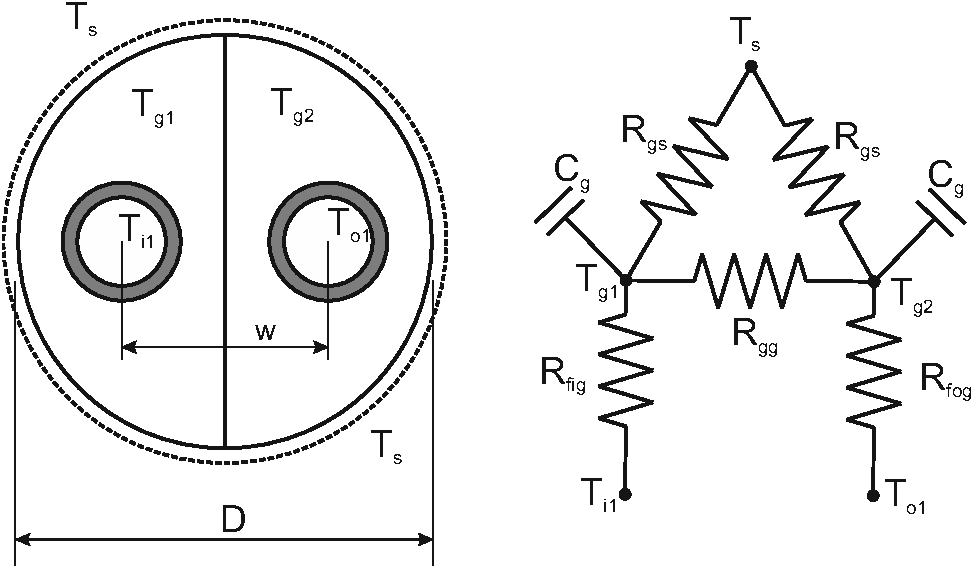
\includegraphics[width=0.8\textwidth]{fig/crosssection_1U}
\end{center}
\caption{Configuration of the 1U type BHE and its corresponding resister-capacitor concept (Reproduced after the FEFLOW book \cite{FEFLOW2014})}
\label{fig:cross_sec_1u}
\end{figure}
%%
\section{Model Concept for BHEs}
To exchange heat with the surrounding soil and rock, borehole heat exchangers have different designs and configurations. The most popular designs can be categorized into 4 differnt types, i.e. the 1U, 2U, CXC and CXA. The U-type BHEs are named after the U shaped tubes laid vertically along the borehole. The number 1 or 2 refer to how many pairs of U tubes are in the same borehole. To illustrate this, Fig \ref{fig:cross_sec_1u} shows the horizontal cross-section of a 1U type BHE. Notice that the U tubes are normally sealed by grout materials, and not in direct contact with the soil. For a typical BHE, a refrigerant fluid is circulating inside of the U tube, absorbing or releasing heat into the surrounding grout and soil. 
%%
In order to numerically simulate the heat transfer inside of a BHE, the device is further conceptualized by the so-called Resister-Capacitor model. This idea originates from the electrical engineering field. In a electrical circuit, if the electric current is hindered by a component, we call this component a Resistor. When a component is capable of storing the electricity, we call it a Capacitor. So the same concept is also applied to the heat transport process in a BHE. Taking the 1U type of BHE in Figure X as an example, there are 4 temperature values assigned to a BHE cross-section at a particular depth. They are $T_s$, $T_{i1}$, $T_{o1}$, $T_{g1}$ and $T_{g2}$, referring to the temperatures of the surrounding soil, the inlet pipe, the outlet pie, the 1st and the 2nd grout zone respectively. As a convention, we always assume the 1st grout zone is the one surrounding the inlet pipe. Following this concept, the heat transfer between the pipe and the soil can be divided into five pathways: i) between inlet pipe and 1st grout zone; ii) between outlet pipe and 2nd grout zone; iii) between 2 grout zones; iv) between 1st grout zone and the soil; v) between 2nd grout zone and the soil. The heat flux $q_n$ on each of these pathways, are driven by the temperature difference and regulated by the heat transfer coefficient $\Phi$. For example, the heat flux from inlet pipe to the 1st grout zone can be calculated by 
\begin{equation}
\label{eqn:heat_transfer}
q_n = \Phi_{fig} \left( T_{i1} - T_{g1} \right), 
\end{equation} 
which is inversely dependent on the product of heat resistance $R$ and specific exchange area $S$
\begin{equation}
\Phi = \frac{1}{R S}
\end{equation}
Depending on the different pathways, we have corresponding heat transfer coefficients, denoted as $\Phi_{fig}$, $\Phi_{fog}$, $\Phi_{gg}$ and $\Phi_{gs}$. Details regarding how to calculate these heat transfer coefficients can be found in the paper of Diersch et al\cite{Diersch2011a}.  
~~\
\section{Governing Equations}
\subsection{Governing Equations for the Heat Transport Process in Soil}
For the heat transport process in the soil, the development of soil temperature $T_s$ is contributed by both the heat convection of the fluid $f$ in the soil and the heat conduction through the soil matrix. Let $\rho^s$, $\rho^f$ and $c^s$, $c^f$ be the density and specific heat capacity of fluid $f$ and soil $s$. If assuming the soil matrix is fully saturated with groundwater, the Darcy velocity of which is described by the vector $q$, then the conservation equation writes as
\begin{equation}
\frac{\partial}{\partial t}  \left[ \epsilon \rho^f c^f + ( 1-\epsilon ) \rho^s c^s \right]  T_s 
+ \nabla \cdot \left(  \rho^f c^f \mathbf{q} T_s  \right) 
- \nabla \cdot \left(  \Lambda^s \cdot \nabla T_s  \right) = H_s,  
\end{equation}
with $\Lambda^s$ the tensor of thermal hydrodynamic dispersion and $H_s$ the source and sink terms for heat. When considering the heat exchange between the BHEs and the soil, the above governing equation is subject to a Cauchy-type of boundary condition: 
\begin{equation}
- \left(  \Lambda^s \cdot \nabla T_s  \right) = q_{n T_s}. 
\end{equation}
\subsection{Governing Equations for the Borehole Heat Exchangers}
The governing equations for the BHE write differently, depending on whether it is for the pipelines or for the grout zones. For the pipelines, the heat transport process is dominated by the convection of the refrigerant. 
\begin{eqnarray}
\label{eqn:gov_eqn_bhe_pipe}
\rho^r c^r \frac{\partial T_k}{\partial t} 
+ \rho^r c^r \mathbf{u} \cdot \nabla T_k 
- \nabla \cdot \left( \Lambda^r \cdot \nabla T_k \right)
&=& H_k \mathrm{~in~} \Omega_k \nonumber \\
\mathrm{with~Cauchy~type~of~BC:~} -\left( \Lambda^r \cdot \nabla T_k \right) \cdot n 
&=& q_{nT_k} \mathrm{~on~} \Gamma_k   \nonumber \\
\mathrm{for~} k &=& i1, o1, (i2, o2) 
\end{eqnarray}
$\Lambda^r$ stands for the hydrodynamic thermodispersion for the refrigerant,  
\begin{equation}
\Lambda^r= \left( \lambda^r + \rho^r c^r \beta_L \| \bm{u} \| \right) \delta. 
\end{equation}
For the grout zones, the heat transport is mainly controlled by the heat dissipation. 
\begin{eqnarray}
\label{eqn:gov_eqn_bhe_grout}
\varepsilon^g \rho^g c^g \frac{\partial T_k}{\partial t} 
- \nabla \cdot \left( \varepsilon^g \lambda^g \cdot \nabla T_k \right)
&=& H_k \mathrm{~in~} \Omega_k \nonumber \\
\mathrm{with~Cauchy~type~of~BC:~} -\left( \varepsilon^g \lambda^g \cdot \nabla T_k \right) \cdot n 
&=& q_{nT_k} \mathrm{~on~} \Gamma_k   \nonumber \\
\mathrm{for~} k &=& g1, (g2, (g3, g4)) 
\end{eqnarray}

\subsection{Calculation of the Cauchy type of Boundary Conditions}
The Cauchy type of boundary conditions exit for the soil part, for the pipelines, and also for the grout zones. They are regulating the heat exchange terms between these zones. In general, the heat exchange flux $q_{nT_k}$ is proportional to the difference of the Temperatures (see Equation \ref{eqn:heat_transfer}). The calculation of these flux terms is summarized in Table \ref{tab:heat_ex_terms}. 

\begin{table}
\centering
\caption{Boundary heat fluxes $q_{nTk}$ for different types of BHEs, reproduced after the FEFLOW book \cite{FEFLOW2014}. }
\label{tab:heat_ex_terms}
\begin{tabular}{p{1cm}p{3cm}p{3cm}p{3cm}p{3cm}}
\hline \hline
k              & 2U & 1U & CXA & CXC \\
\hline \hline
\multirow{2}{*}{i1}    & $-\Phi_{fig}^{2U}(T_{g1}-T_{i1})$ 
                       & $-\Phi_{fig}^{1U}(T_{g1}-T_{i1})$  
                       & $-\Phi_{fig}^{CXA}(T_{g1}-T_{i1})$
                       & $-\Phi_{ff}^{CXC}(T_{o1}-T_{i1})$ \\
                       & & & $-\Phi_{ff}^{CXA}(T_{o1}-T_{i1})$ & \\
\hline
i2             & $-\Phi_{fig}^{2U}(T_{g2}-T_{i2})$
               & -  & -  & - \\
\hline
\multirow{2}{*}{o1}    & $-\Phi_{fog}^{2U}(T_{g3}-T_{o1})$
                       & $-\Phi_{fog}^{1U}(T_{g2}-T_{o1})$  
                       & $-\Phi_{ff}^{CXA}(T_{i1}-T_{o1})$               
                       & $-\Phi_{fog}^{CXC}(T_{g1}-T_{o1})$ \\
                       & & & & $-\Phi_{ff}^{CXC}(T_{i1}-T_{o1})$\\
\hline
o2             & $-\Phi_{fog}^{2U}(T_{g4}-T_{o2})$
               & -  & -  & - \\
\hline
\multirow{5}{*}{g1}    & $-\Phi_{gs}^{2U}(T_{s}-T_{g1})  $ & $-\Phi_{gs}^{1U}(T_{s}-T_{g1})$     
               & $-\Phi_{gs}^{CXC}(T_{s}-T_{g1})$ & $-\Phi_{gs}^{CXA}(T_{s}-T_{g1})$ \\   
                       & $-\Phi_{fig}^{2U}(T_{i1}-T_{g1})$ & $-\Phi_{fig}^{1U}(T_{i1}-T_{g1})$  
               & $-\Phi_{fog}^{CXC}(T_{o1}-T_{g1})$ & $-\Phi_{gs}^{CXA}(T_{s}-T_{g1})$ \\
                       & $-\Phi_{gg2}^{2U}(T_{g2}-T_{g1})$ & $-\Phi_{gg}^{1U}(T_{g2}-T_{g1})$    &-&-\\
                       & $-\Phi_{gg1}^{2U}(T_{g3}-T_{g1})$ &                                     &~&~\\
                       & $-\Phi_{gg1}^{2U}(T_{g4}-T_{g1})$ &                                     &~&~\\
\hline
\multirow{5}{*}{g2}    & $-\Phi_{gs}^{2U}(T_{s}-T_{g2})$   & $-\Phi_{gs}^{1U}(T_{s}-T_{g2})$     &~&~\\ 
                       & $-\Phi_{fig}^{2U}(T_{i2}-T_{g2})$ & $-\Phi_{fog}^{1U}(T_{o1}-T_{g2})$   &~&~\\
                       & $-\Phi_{gg2}^{2U}(T_{g1}-T_{g2})$ & $-\Phi_{gg}^{1U}(T_{g1}-T_{g2})$    &-&-\\
                       & $-\Phi_{gg1}^{2U}(T_{g3}-T_{g2})$ &                                     &~&~\\
                       & $-\Phi_{gg1}^{2U}(T_{g4}-T_{g2})$ &                                     &~&~\\
\hline
\multirow{5}{*}{g3}    & $-\Phi_{gs}^{2U}(T_{s}-T_{g3})$   &                                     &~&~\\
                       & $-\Phi_{fig}^{2U}(T_{o1}-T_{g3})$ &                                     &~&~\\
                       & $ -\Phi_{gg2}^{2U}(T_{g4}-T_{g3})$&-                                    &-&-\\
                       & $-\Phi_{gg1}^{2U}(T_{g1}-T_{g3})$ &                                     &~&~\\
                       & $-\Phi_{gg1}^{2U}(T_{g2}-T_{g3})$ &                                     &~&~\\
\hline
\multirow{5}{*}{g4}    & $-\Phi_{gs}^{2U}(T_{s}-T_{g4})$   &                                     &~&~\\
                       & $-\Phi_{fig}^{2U}(T_{o2}-T_{g4})$ &                                     &~&~\\
                       & $-\Phi_{gg2}^{2U}(T_{g3}-T_{g4})$ &-                                    &-&-\\
                       & $-\Phi_{gg1}^{2U}(T_{g1}-T_{g4})$ &                                     &~&~\\
                       & $-\Phi_{gg1}^{2U}(T_{g2}-T_{g4})$ &                                     &~&~\\
\hline \hline
\end{tabular}
\end{table}

\section{Numerical Model}
%%
\begin{figure}
\begin{center}
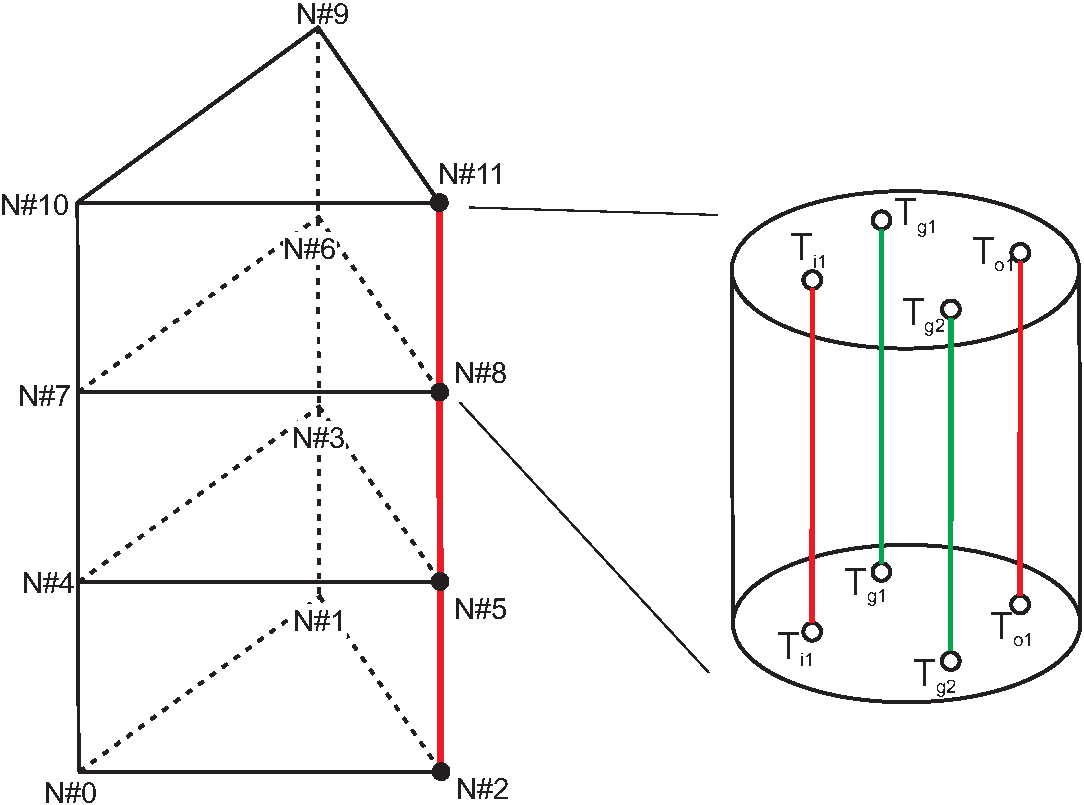
\includegraphics[width=0.8\textwidth]{fig/simple_mesh_geometry}
\end{center}
\caption{Mesh and geometry structure, with soil domain represented by prism elements and BHE by line elements. }
\label{fig:simple_mesh}
\end{figure}
%%

\subsection{Mesh Arrangement}
To simulate the heat transport process together with BHEs, a dual-continuum approach has been adopted to treat the soil and BHEs part respectively. For the soil part, prism elements are used to discretize the 3D domain. In addition to that, 1D line elements along the edge of the prism elements are chosen to form the 2nd domain, representing BHEs. The example illustrated in Figure \ref{fig:simple_mesh} contains a mesh structure with 12 nodes and 6 element. Node "0" - "11" forms the 3 prism elements, which refers to the the soil domain. The BHE domain is composed of 3 line elements in red color. Notice the node "2", "5", "8" and "11" are both employed by the prim and the line elements. As a result, the total number of nodes remains the same and the number of elements slightly increases. In soil domain, there is only one primary variable, the soil temperature, on each node. While in the BHE domain, each node has 4, 8, or 3 primary variables, depending on the type of the BHE. Table \ref{tab:bhe_primary_variables} summarizes these combinations. 
%%
\begin{table}
\caption{Different combination of primary variables for the borehole heat exchangers. }
\label{tab:bhe_primary_variables}
\centering
\begin{tabular}{l l l}
\hline
Type of BHE    & Number of Primary Variables & Combination of Primary Variables \\
\hline
1U             & 4 & $\mathrm{T_{i1},~T_{o1},~T_{g1},~T_{g2}}$\\
2U             & 8 & $\mathrm{T_{i1},~T_{i2},~T_{o1},~T_{o2},~T_{g1},~T_{g2},~T_{g3},~T_{g4}}$\\
CXA            & 3 & $\mathrm{T_{i1},~T_{o1},~T_{g1}}$\\
CXC            & 3 & $\mathrm{T_{i1},~T_{o1},~T_{g1}}$ \\
\hline
\end{tabular}
\end{table}

The following text box shows the content of the mesh file for OpenGeoSys. Under the key word \textit{\$NODES}, the number \textit{12} tells the software there are all together 12 nodes. This is followed by a section of node coordinate information. Each node begins with a index number, then the x, y, and z coordinates. The keyword \$ELEMENTS signals the begin of element information. Here we have 6 elements, with 3 prisms and 3 lines. Similar to the node information, each element begins with an index value, then a second index linking to the corresponding material properties. The keywords \textit{pris} and \textit{line} reflects the type of the element, followed by the index of nodes that are connected to this element. 
%%
\begin{Verbatim}[gobble=0, 
                 frame=single, 
                 label=Mesh File, 
                 numbers=left]
#FEM_MSH
 $PCS_TYPE
  GROUNDWATER_FLOW
 $NODES
  12 
0 0 0 0
1 0 1 0
2 1 0 0
3 0 1 1
4 0 0 1
5 1 0 1
6 0 1 2
7 0 0 2
8 1 0 2
9 0 1 3
10 0 0 3
11 1 0 3
  $ELEMENTS
  6 
0 0 pris 2 1 0 5 3 4
1 0 pris 5 3 4 8 6 7
2 0 pris 8 6 7 11 9 10 
3 1 line 9 6
4 1 line 6 3
5 1 line 3 1
#STOP
\end{Verbatim}

\subsection{Finite Element Discretization}
For the domain of BHEs, the governing equations \ref{eqn:gov_eqn_bhe_pipe} and \ref{eqn:gov_eqn_bhe_grout} are discretized by finite elements. If introducing the spatial weighting function $\omega$, the weak statements wirte as
\begin{eqnarray}
\label{eqn:gov_eqn_bhe_pipe_dis}
\int_{\Omega_k} \left[ \omega \rho^r c^r \left( \frac{\partial T_k}{\partial t} + \bm{u} \cdot \nabla T_k \right) + \nabla \omega \cdot \left( \Lambda^r \cdot \nabla T_k \right) \right] d\Omega &=&~ \nonumber\\
-\int_{\Gamma_k} \omega q_{nT_k} d\Gamma_k + \int_{\Omega_k} \omega H_k d\Omega &~& \mathrm{~for~k~}=~i1,~o1,~(i2,~o2)
\end{eqnarray}
for the pipelines, and 
\begin{eqnarray}
\label{eqn:gov_eqn_bhe_grout_dis}
\int_{\Omega_k} \left[ \omega \rho^g c^g \frac{\partial T_k}{\partial t} + \nabla \omega \cdot \left( \Lambda^g \cdot \nabla T_k \right) \right] d\Omega &=&~ \nonumber\\
-\int_{\Gamma_k} \omega q_{nT_k} d\Gamma_k + \int_{\Omega_k} \omega H_k d\Omega &~& \mathrm{~for~k~}=~g1,~(g2,~(g3,~g4))
\end{eqnarray}
for the grout zones. If using Galerkin Finite Element Method (GFEM), the above equation \ref{eqn:gov_eqn_bhe_pipe_dis} and \ref{eqn:gov_eqn_bhe_grout_dis} can be written in the matrix form. 
\begin{equation}
\bm{P}^\pi \cdot \bm{\dot{T}}^\pi + ( \bm{L^\pi} + \bm{R^\pi} ) \cdot \bm{T^\pi} = \bm{W}^\pi - \bm{R}^{\pi s} \cdot \bm{T}^{s}
\end{equation}
with the time derivative related mass matrix $\bm{P}^\pi$ formulated as
\begin{equation}
\bm{P}^\pi = \left\{ \begin{array}{ll}
\left( \begin{array}{cccccccc}
\bm{P}_{i1} & 0 & 0 & 0 & 0 & 0 & 0 & 0 \\
0 & \bm{P}_{i2} & 0 & 0 & 0 & 0 & 0 & 0 \\
0 & 0 & \bm{P}_{o1} & 0 & 0 & 0 & 0 & 0 \\
0 & 0 & 0 & \bm{P}_{o2} & 0 & 0 & 0 & 0 \\
0 & 0 & 0 & 0 & \bm{P}_{g1} & 0 & 0 & 0 \\
0 & 0 & 0 & 0 & 0 & \bm{P}_{g2} & 0 & 0 \\
0 & 0 & 0 & 0 & 0 & 0 & \bm{P}_{g3} & 0 \\
0 & 0 & 0 & 0 & 0 & 0 & 0 & \bm{P}_{g4} \end{array} \right)
  & \mbox{2U} \\
\left( \begin{array}{cccc}
\bm{P}_{i1} & 0 & 0 & 0  \\
0 & \bm{P}_{o1} & 0 & 0  \\
0 & 0 & \bm{P}_{g1} & 0  \\
0 & 0 & 0 & \bm{P}_{g2}  \end{array} \right)
 & \mbox{1U} \\
\left( \begin{array}{ccc}
\bm{P}_{i1} & 0 & 0  \\
0 & \bm{P}_{o1} & 0  \\
0 & 0 & \bm{P}_{g1}  \end{array} \right)
 & \mbox{CXA or CXC. } \\
       \end{array} \right.
\end{equation}
For the pipeline or grout zone of the BHE, the mass matrix writes
\begin{equation}
\bm{P}_k = \left\{ \begin{array}{rcl}
\Sigma_{e} \int_{\Omega_k^e} \rho^r c^r N_i N_j d\Omega^e 
   &\mbox{~for~}& k = i1, o1, (i2, o2) \\
\Sigma_{e} \int_{\Omega_k^e} \rho^g c^g N_i N_j d\Omega^e 
   &\mbox{~for~}& k = g1, (g2, (g3, g4)). 
       \end{array} \right.
\end{equation}
The heat exchange terms are summarized in the matrix $\bm{R}^\pi$, 
\begin{equation}
\label{eqn:heat_exchange_term_R}
\bm{R}^\pi = \left\{ \begin{array}{ll}
\scalemath{0.5}{
\left( \begin{array}{cccccccc}
\bm{R}_{i1} + \bm{R}_{io} & 0 & -\bm{R}_{io} & 0 & -\bm{R}_{i1} & 0 & 0 & 0 \\
0 & \bm{R}_{i2} & 0 & 0 & 0 & -\bm{R}_{i2} & 0 & 0 \\
-\bm{R}_{io} & 0 & \bm{R}_{io} + \bm{R}_{o1} & 0 & 0 & 0 & -\bm{R}_{o1} & 0 \\
0 & 0 & 0 & \bm{R}_{o2} & 0 & 0 & 0 & -\bm{R}_{o2} \\
-\bm{R}_{i1} & 0 & 0 & 0 & \bm{R}_{i1}+2\bm{R}_{g1}+\bm{R}_{g2}+\bm{R}_{s} & -\bm{R}_{g2} & -\bm{R}_{g1} & -\bm{R}_{g1} \\
0 & -\bm{R}_{i2} & 0 & 0 & -\bm{R}_{g2} & \bm{R}_{i2}+2\bm{R}_{g1}+\bm{R}_{g2}+\bm{R}_{s} & -\bm{R}_{g1} & -\bm{R}_{g1} \\
0 & 0 & -\bm{R}_{o1} & 0 & -\bm{R}_{g1} & -\bm{R}_{g1} & \bm{R}_{o1}+2\bm{R}_{g1}+\bm{R}_{g2}+\bm{R}_{s} & 0 \\
0 & 0 & 0 & -\bm{R}_{o2} & -\bm{R}_{g1} & -\bm{R}_{g1} & -\bm{R}_{g2} & \bm{R}_{o2}+2\bm{R}_{g1}+\bm{R}_{g2}+\bm{R}_{s} \end{array} \right)
}
  & \mbox{2U} \\
\scalemath{0.7}{
\left( \begin{array}{cccc}
\bm{R}_{i1}+\bm{R}_{io} & -\bm{R}_{io} & -\bm{R}_{i1} & 0  \\
-\bm{R}_{io} & \bm{R}_{o1}+\bm{R}_{io} & 0 & -\bm{R}_{o1}  \\
-\bm{R}_{i1} & 0 & \bm{R}_{i1}+\bm{R}_{g1} & -\bm{R}_{g1}  \\
0 & -\bm{R}_{o1} & -\bm{R}_{g1} & \bm{R}_{o1}+\bm{R}_{g1}  \end{array} \right)
}
 & \mbox{1U} \\
\scalemath{0.7}{
\left( \begin{array}{ccc}
\bm{R}_{i1}+\bm{R}_{io} & -\bm{R}_{io} & -\bm{R}_{i1}  \\
-\bm{R}_{io} & \bm{R}_{io} & 0  \\
-\bm{R}_{i1} & 0 & \bm{R}_{i1}  \end{array} \right)
}
 & \mbox{CXA} \\
\scalemath{0.7}{
\left( \begin{array}{ccc}
\bm{R}_{io} & -\bm{R}_{io} & 0  \\
-\bm{R}_{io} & \bm{R}_{io}+\bm{R}_{o1} & -\bm{R}_{o1}  \\
0 & -\bm{R}_{o1} & \bm{R}_{o1}  \end{array} \right)
}
 & \mbox{CXA} 
       \end{array} \right.
\end{equation}
\begin{equation}
\bm{L}^\pi = \left\{ \begin{array}{ll}
\left( \begin{array}{cccccccc}
\bm{L}_{i1} & 0 & 0 & 0 & 0 & 0 & 0 & 0 \\
0 & \bm{L}_{i2} & 0 & 0 & 0 & 0 & 0 & 0 \\
0 & 0 & \bm{L}_{o1} & 0 & 0 & 0 & 0 & 0 \\
0 & 0 & 0 & \bm{L}_{o2} & 0 & 0 & 0 & 0 \\
0 & 0 & 0 & 0 & \bm{L}_{ig} & 0 & 0 & 0 \\
0 & 0 & 0 & 0 & 0 & \bm{L}_{ig} & 0 & 0 \\
0 & 0 & 0 & 0 & 0 & 0 & \bm{L}_{og} & 0 \\
0 & 0 & 0 & 0 & 0 & 0 & 0 & \bm{L}_{og} \end{array} \right)
  & \mbox{2U} \\
\left( \begin{array}{cccc}
\bm{L}_{i1} & 0 & 0 & 0  \\
0 & \bm{L}_{o1} & 0 & 0  \\
0 & 0 & \bm{L}_{g1} & 0  \\
0 & 0 & 0 & \bm{L}_{g2}  \end{array} \right)
 & \mbox{1U} \\
\left( \begin{array}{ccc}
\bm{L}_{i1} & 0 & 0  \\
0 & \bm{L}_{o1} & 0  \\
0 & 0 & \bm{L}_{g1}  \end{array} \right)
 & \mbox{CXA or CXC} \\
       \end{array} \right.
\end{equation}
For the pipeline part, the transport operator $L$ is composed of both advection and dispersion terms, 
\begin{equation}
\begin{array}{lll}
\bm{L}_k = \Sigma_{e} \int_{\Omega_k^e} \left( N_i \rho^r c^r \nabla N_j 
+ \nabla N_i \cdot ( \Lambda \cdot \nabla N_j ) \right) d\Omega^e 
&\mbox{~for~}& k = i1, o1, (i2, o2). 
\end{array}
\end{equation}
While for the grout zones, only the heat dissipation terms contribute, 
\begin{equation}
\begin{array}{lll}
\bm{L}_{ig} = \bm{L}_{og} = \Sigma_{e} \int_{\Omega_k^e} \nabla N_i \cdot ( \Lambda^g \cdot \nabla N_j ) d\Omega^e 
&\mbox{~for~}& k = (g1, g2, g3, g4). 
\end{array}
\end{equation}
For the source and sink terms, 
\begin{equation}
\begin{array}{lll}
\bm{W}_{k} = \Sigma_{e} \int_{\Omega_k^e} N_i H_k d\Omega^e 
&\mbox{~for~}& \forall k. 
\end{array}
\end{equation}
For the heat exchange terms $\bm{R_{\pi s}}$ and $\bm{R_{s \pi}}$, 
\begin{equation}
\bm{R}^{s \pi} = {\bm{R}^{\pi s}}^{T} = \left\{ \begin{array}{ll}
(\bm{0}~\bm{0}~\bm{0}~\bm{0}~\bm{-R_s}~\bm{-R_s}~\bm{-R_s}~\bm{-R_s}) 
   & \mbox{~~2U} \\
(\bm{0}~\bm{0}~\bm{-R_s}~\bm{-R_s}) 
   & \mbox{~~1U} \\
(\bm{0}~\bm{0}~\bm{-R_s}) 
   & \mbox{~~CXA or CXC} 
       \end{array} \right.
\end{equation}
\subsection{Assembly of the Global Equation System}



\subsection{Picard Iterations and Time Step Schemes}

%Implementation
\chapter{Implementation with OpenGeoSys}

\section{Process Definition and Primary Variables}

\section{Memory Space for Global Equation System}

\section{Local Assembly of BHEs}

\section{Imposing Boundary Conditions}

\section{Output of Pipe Temperatures}

%Setting up a model with one BHE
\chapter{Running Heat Transport model with BHEs}

\section{Download and compile the source code}
Currently, the BHE feature is developed in a separate branche of OpenGeoSys, to isolate it from changes of the main OGS development. Once this document is finished and the code is fully verified, it will be merged into the OpenGeoSys main branche and released to the public. For interested readers who would like to have a first look, the code can be downloaded from the following link. 
\par
\url{https://github.com/HaibingShao/ogs5-trunk.git}
\par
Most of the changes are kept under the branch \texttt{borehole\_heat\_exchanger}, and they will be constantly merged into the main branch "develop". 

\subsection{Download the source code}
If you are using the Git command line interface, the code can be obtained by typing in the command line prompt as follows.  
\begin{Verbatim}
C:\haibing_working\ogs>git clone https://github.com/HaibingShao/ogs5-trunk.git
\end{Verbatim}
Or, if you prefer a GUI, I personally recommend to use SourceTree on the Windows platform. After a fresh installation of the software SourceTree, the following interface will appear. 
%%
\begin{figure}
\begin{center}
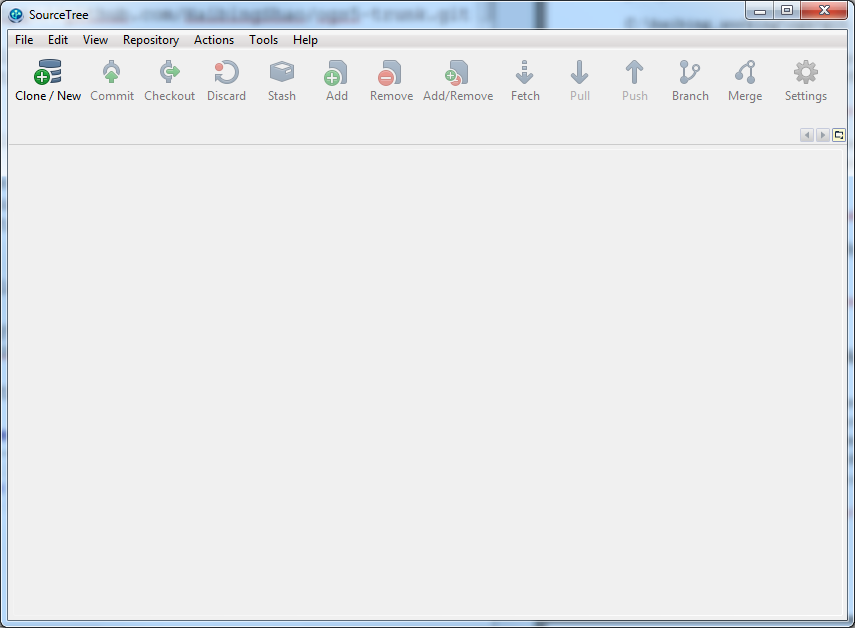
\includegraphics[width=0.8\textwidth]{fig/sourcetree_initial}
\end{center}
\caption{SourceTree window as in the initial stage.}
\label{fig:sourcetree_initial}
\end{figure}
%%
Clicking the button Clone/New in the upper-left corner, you will be asked to give the location of repository. You may use the Github link provided above, or first fork from the above repository and clone from your own repository on Github. 
%%
\begin{figure}
\begin{center}
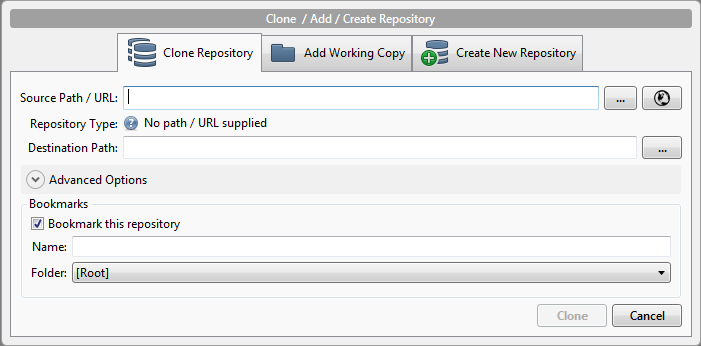
\includegraphics[width=0.6\textwidth]{fig/sourcetree_repo_dialog}
\end{center}
\caption{SourceTree dialog asking for the location of the repository}
\label{fig:sourcetree_repo_dialog}
\end{figure}
%%
After the code has been successfully cloned to your own computer, you will see all history of the development in SourceTree as follows. 
%%
\begin{figure}
\begin{center}
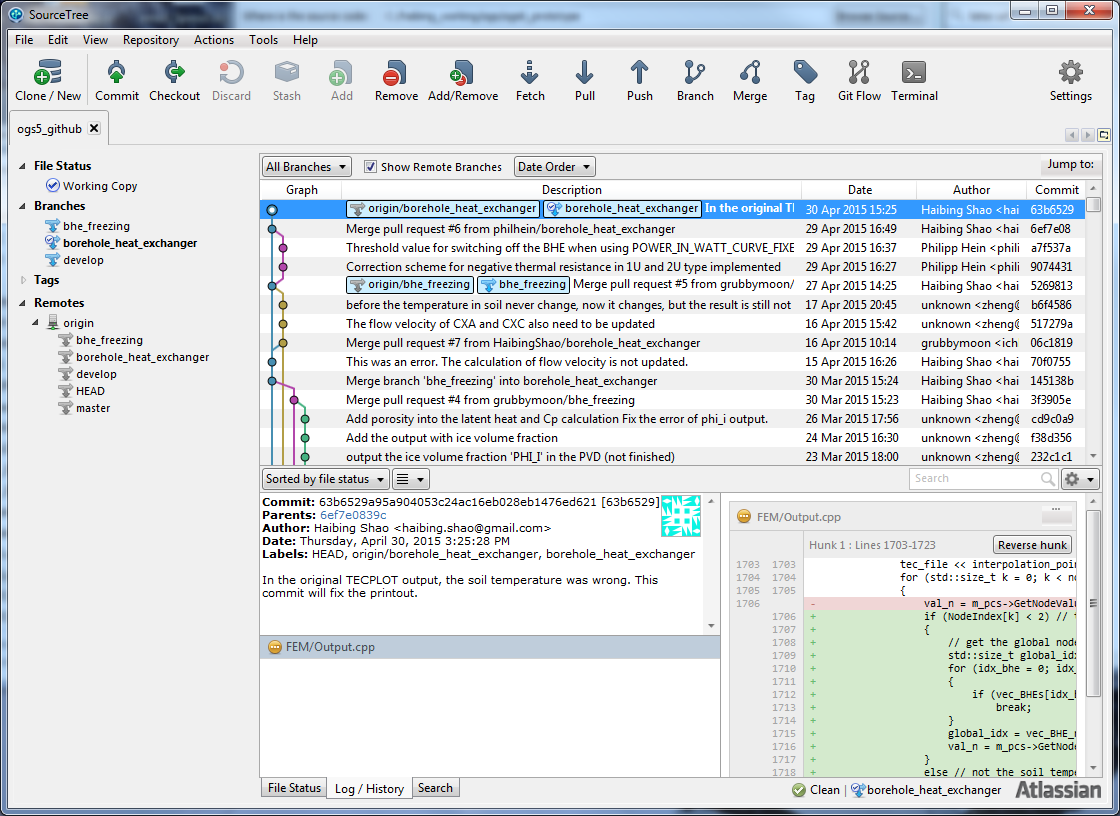
\includegraphics[width=0.8\textwidth]{fig/sourcetree_repo}
\end{center}
\caption{SourceTree window with detailed history of a repository.}
\label{fig:sourcetree_repo}
\end{figure}
%%

\subsection{Using CMake to configure the building project}
Before the compilation of the source code, we need to use the software CMake to generate the configuration and makefiles which are specific to the building environment. Here I am taking CMake version 2.8.12.2 as an example. In the following figure, Cmake GUI was freshly started. First, one needs to define two paths in the CMake GUI. The first one is the folder where the source code of OpenGeoSys is located. The second path refers to the folder where the make files will be generated. 
%%
\begin{figure}
\begin{center}
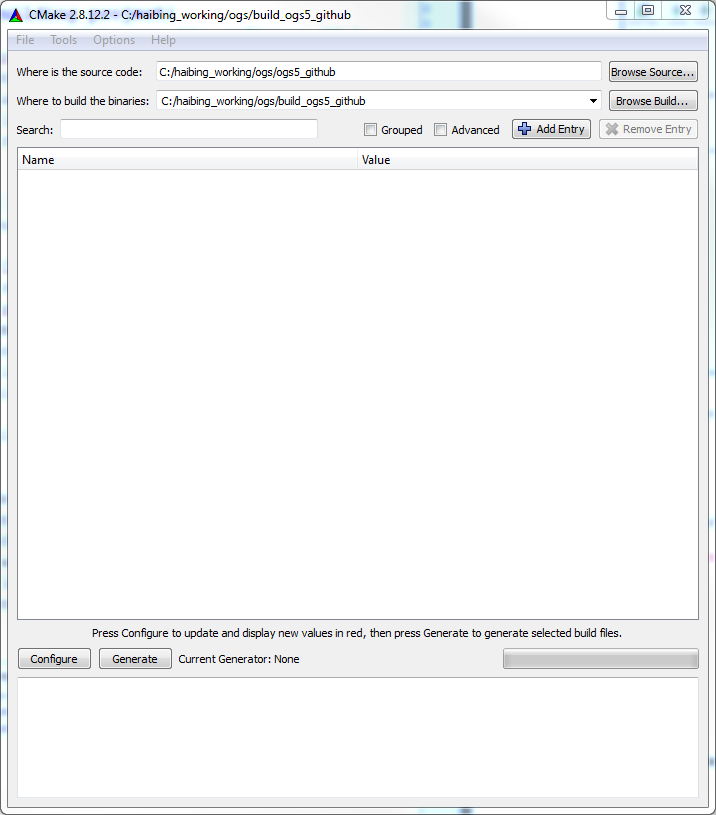
\includegraphics[width=0.6\textwidth]{fig/cmake_initial}
\end{center}
\caption{CMake interface of configuring the build information. }
\label{fig:cmake_initial}
\end{figure}
%%
After clicking on the "Configure" button, CMake will ask several questions, depending on different types of operating system and the compiling tools. In my case, I choose the "Visual Studio 2013 x86" option. Once the configuration has finished, the build options will be demonstrated in the CMake GUI. To build the OpenGeoSys code with BHE features, one only needs to choose the \texttt{OGS\_FEM} option. Finally, once clicking on the "Generate" button, CMake will prepare all makefiles in the build folder. 
%%
\begin{figure}
\begin{center}
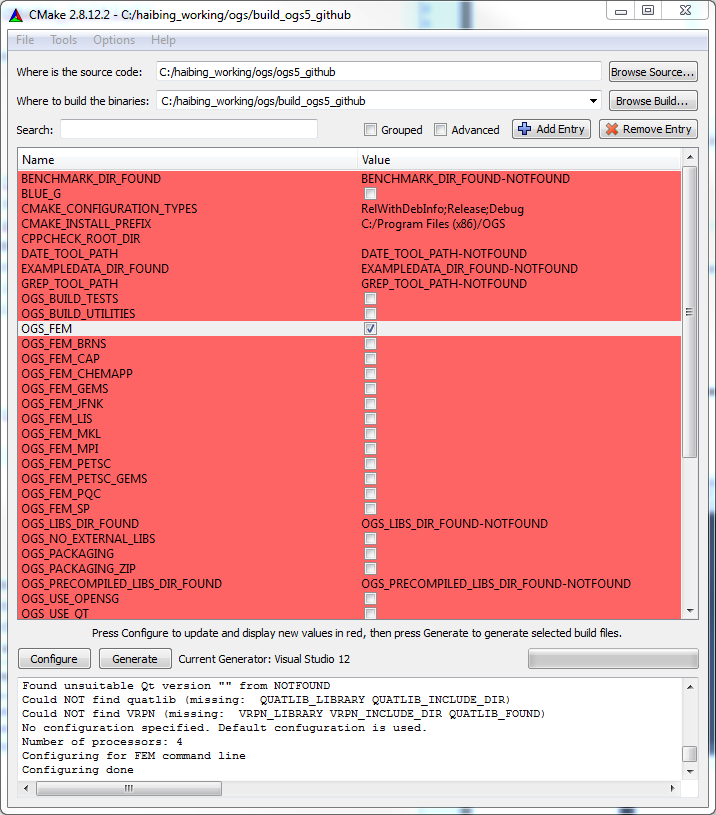
\includegraphics[width=0.6\textwidth]{fig/cmake_configured}
\end{center}
\caption{CMake interface showing different building options. }
\label{fig:cmake_configured}
\end{figure}
%%
\subsection{Compiling the code}
As the author is mainly developing the code with Visual Studio 2013 Express version, the building process will be demonstrated with the same software. Provided the configuration was accomplished by CMake successfully in the previous step, there will be a file named with "OGS.sln" in the build file. Opening this file with Visual Studio will import source code and building configurations into the development environment. 
%%
\begin{figure}
\begin{center}
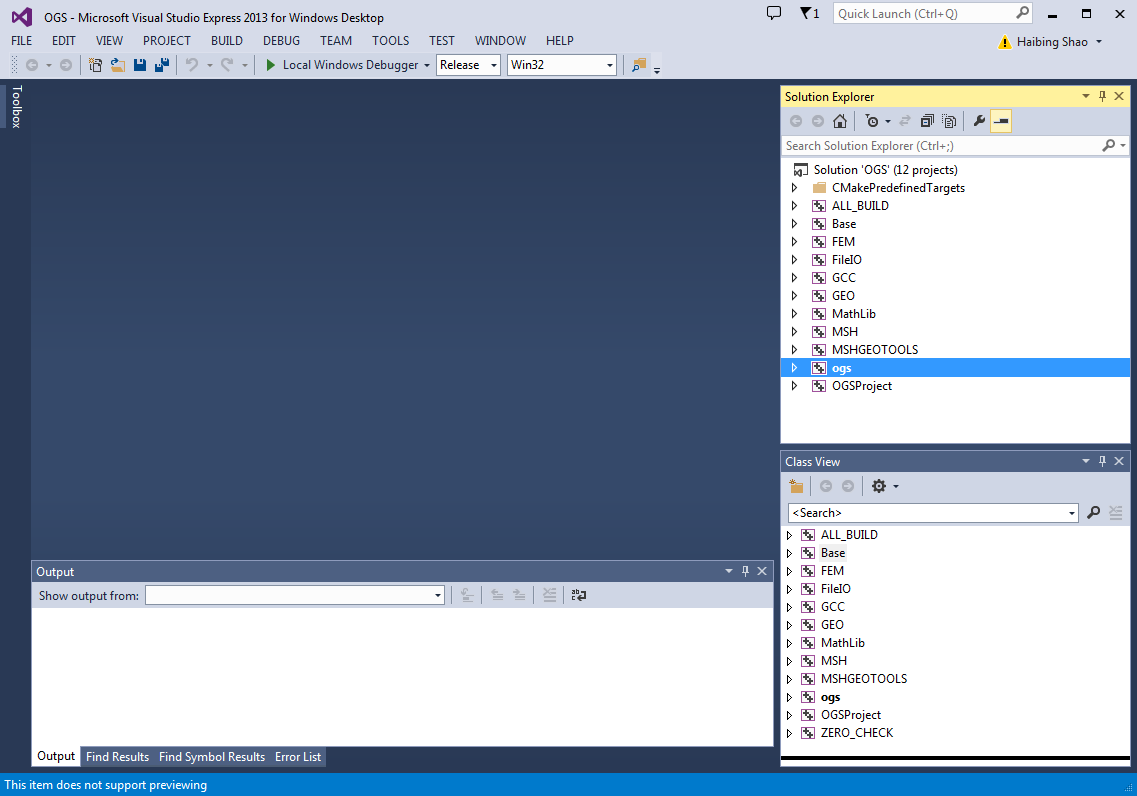
\includegraphics[width=0.8\textwidth]{fig/vs2013exp_ogs}
\end{center}
\caption{Visual Studio interface after opening the OpenGeoSys solution file. }
\label{fig:vs2013exp_ogs}
\end{figure}
%%
To build the source code, choose from the file menu "BUILD", and then click on the first option "Build Solution". It takes a couple of minutes to run the full building process for the first time. After it is finished, the executable files will be found under the bin Debug or bin Release folder, depending on which building mode was chosen. 

\section{Define Heat Transport Process with BHEs}

In the last section, the OpenGeoSys code was successfully compiled and an ogs.exe executable file has been built. In this section, we will introduce the process of setting up a modeling project to simulate heat transport process with borehole heat exchangers.  

\subsection{Process Definition}

Originally, the heat transport simulation in an OpenGeoSys project is performed by defining the process as \texttt{HEAT\_TRANSPORT}. To include the interaction with BHEs, we have introduced a new process named as "\texttt{HEAT\_TRANSPORT\_BHE}". In the following, a PCS file is introduced, with one \texttt{GROUNDWATER\_FLOW} and one \texttt{HEAT\_TRANSPORT\_BHE} process defined in it. 

\begin{Verbatim}[gobble=0, 
                 frame=single, 
                 label=PCS File Definition including Interaction with Borehole Heat Exchangers, 
                 numbers=left]
#PROCESS
 $PCS_TYPE
  GROUNDWATER_FLOW
 $DEACTIVATED_SUBDOMAIN
  1
  1 
#PROCESS
 $PCS_TYPE
  HEAT_TRANSPORT_BHE
 $PRIMARY_VARIABLE
  TEMPERATURE_SOIL
 $BOUNDARY_CONDITION_OUTPUT
#STOP
\end{Verbatim}

\subsection{Deactivated Sub-domains}
In the above PCS file, some readers might have already noticed that there are two numbers given under the key word \texttt{\$DEACTIVATED\_SUBDOMAIN}. The first number "1" on line \#7 means there is one sub-domain deactivated for the \texttt{GROUNDWATER\_FLOW} process, and the second number "1" on line \#8 tells the index of this deactivated domain. So why does the sub-domain "1" need to be turned off? This is because the sub-domain "0" in this project is referring to the soil matrix, while the sub-domain "1" is the borehole heat exchanger. Since the BHE is grouted and impermeable, it is not necessary to calculate groundwater flow through a BHE. Therefore its representative sub-domain is deactivated. 

\subsection{Primary Variables}

From the section \ref{sec:model_concept} and \ref{sec:gov_eqns}, we know that there are multiple primary variables applied in the BHE simulation. In the soil sub-domain primary variable is the soil temperature, while on the BHE they are the temperatures of inlet outlet pipes and their surrounding grout zones. The key words used for these processes, are summerized in Table \ref{tab:pvar_keywords}. In section \ref{sec:temp_output}, when the output is configured, these key words will be used. 

\begin{table}
\caption{Key words used in OGS BHE project for different primary variables. }
\label{tab:pvar_keywords}
\centering
\begin{tabular}{l l }
\hline
Symbols    & Key words  \\
\hline
$T_s$             & \texttt{TEMPERATURE\_SOIL} \\
$T_{i1}$          & \texttt{TEMPERATURE\_IN\_1} \\
$T_{i2}$          & \texttt{TEMPERATURE\_IN\_2} \\
$T_{o1}$          & \texttt{TEMPERATURE\_OUT\_1} \\
$T_{o2}$          & \texttt{TEMPERATURE\_OUT\_1} \\
$T_{g1}$          & \texttt{TEMPERATURE\_G\_1} \\
$T_{g2}$          & \texttt{TEMPERATURE\_G\_2} \\
$T_{g3}$          & \texttt{TEMPERATURE\_G\_3} \\
$T_{g4}$          & \texttt{TEMPERATURE\_G\_4} \\
\hline
\end{tabular}
\end{table}

\section{Geometry of BHEs}

\begin{Verbatim}[gobble=0, 
                 frame=single, 
                 label=Geometry Definition in the GLI File of an OpenGeoSys Project, 
                 numbers=left]
#POINTS
0  0.0 0.0  18.32 $NAME POINT0
1  1.8 0.0  18.32 $NAME POINT1  
2  1.8 1.8  18.32 $NAME POINT2  
3  0.0 1.8  18.32 $NAME POINT3  
4  0.9 0.9  18.32 $NAME POINT4  
5  0.0 0.0  0.0   $NAME POINT5
6  1.8 0.0  0.0   $NAME POINT6  
7  1.8 1.8  0.0   $NAME POINT7  
8  0.0 1.8  0.0   $NAME POINT8  
9  0.9 0.9  0.0   $NAME POINT9  
10 1.14 0.9  18.32 $NAME POINT10  
11 1.14 0.9  0.0   $NAME POINT11  
12 1.34 0.9  18.32 $NAME POINT12  
13 1.34 0.9  0.0   $NAME POINT13
14 1.55 0.9  18.32 $NAME POINT14  
15 1.55 0.9  0.0   $NAME POINT15
16 1.75 0.9  18.32 $NAME POINT16  
17 1.75 0.9  0.0   $NAME POINT17
#POLYLINE
 $NAME
  BHE_1
 $POINTS
   4
   9
#STOP
\end{Verbatim}

As shown in the GLI file above,  "\texttt{BHE\_1}" is refering to a polyline composed of point \#4 and point \#9. To define different BHEs, each BHE in the model has to be given a different polyline in the geometry definition. The geometry names will be used later in the MMP and OUT file as a reference of different BHEs. 

\section{Mesh of BHEs}



\section{Parameters of BHEs}



\section{Output of Temperatures in the BHEs}
\label{sec:temp_output}


\section{Visualization of the Temperatures Evolution}

\subsection{Visualization of Soil Temperatures}

\subsection{Visualization of BHE Temperatures}




%Model Verificationa and Validation
\chapter{Model Verification and Validation}

\section{Outflow Temperature Development} % FEFLOW model

\section{Thermal Response Test (TRT)} % 

\section{Soil Temperature Distribution} % line source model





%Applications
\chapter{Applications}

\renewcommand{\indexname}{Keyword index}
\printindex

\cleardoublepage
\bibliographystyle{plain}
\bibliography{common_bib_file}


\end{document}